
\documentclass[12pt]{article}
\usepackage[T1]{fontenc}
\usepackage{hyperref}
\usepackage{amsmath}
\usepackage{graphicx}
\usepackage{tikz, mhchem}
\usepackage{mathtools}

\setcounter{figure}{0}

\title{Free Amino Acids dynamics over time in Human Milk}
% \author{Federico J. Zertuche}
% \date{\today}

\begin{document}
\maketitle

\begin{abstract}
%Holá \ldots
\end{abstract}

\section{Free amino acid Composition of HM over time}

Change of concentration over time is studied for each of the AA recorded. They are divided into two categories:

\begin{itemize}
  \item[Essential:] HIS, ILE, LEU, LYS, MET, PHE, THR, TRP, VAL.
  \item[Non Essential:] ALA, ARG, ASN, ASP, CYS, GLN, GLU, GLY, PRO, SER, TYR.
\end{itemize}

\subsection{Distribution over time}

Figures \ref{fig:distE} and \ref{fig:distNE} show the concentration of each AA over time. In most cases concentration increases over time.

Trends in time are not clear by looking at the tables and density plots. The following regression model is fitted to study this relationship:

\begin{equation}
  AA = \alpha_0 + \alpha_1 \ week + \alpha_{id}
\end{equation}

where the effect $\alpha_{id}$ is different for each participant.

\begin{figure}[ht]\label{fig:EAA_W_coeff}
  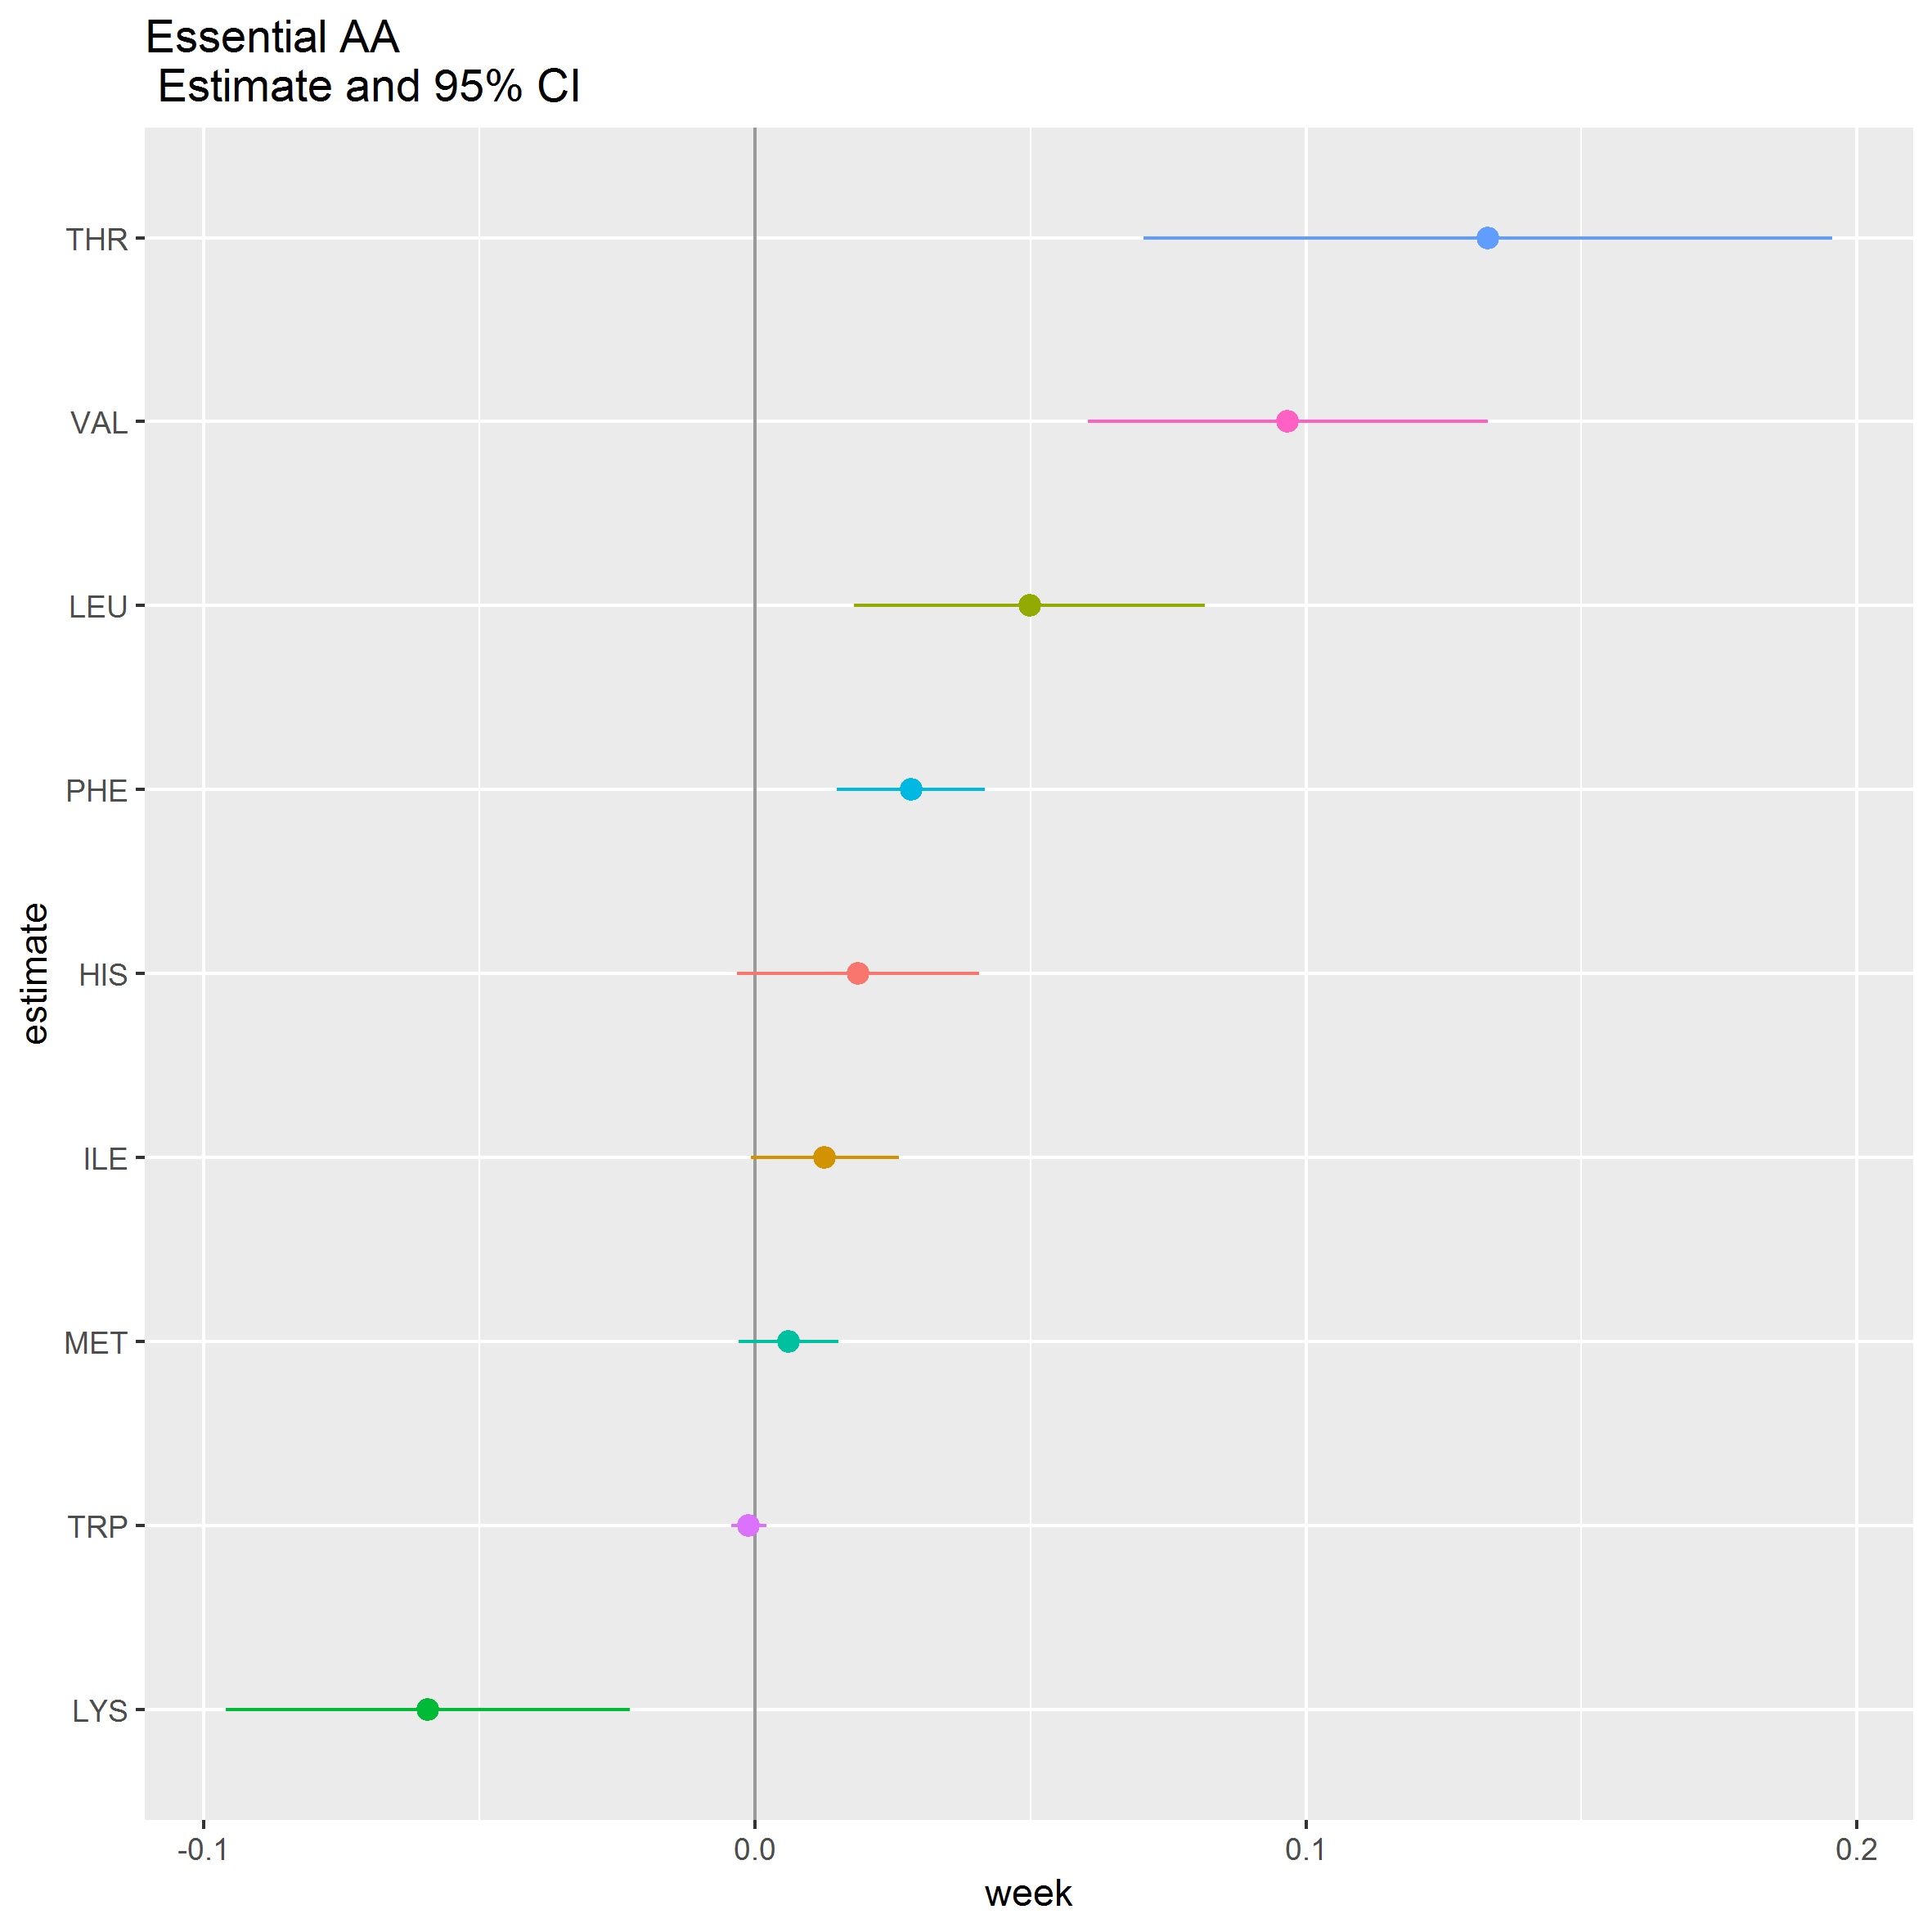
\includegraphics[width= \textwidth]{../week/EAA_W_coeff.png}
  \caption{}
\end{figure}

\begin{figure}[ht]\label{fig:NEAA_W_coeff}
  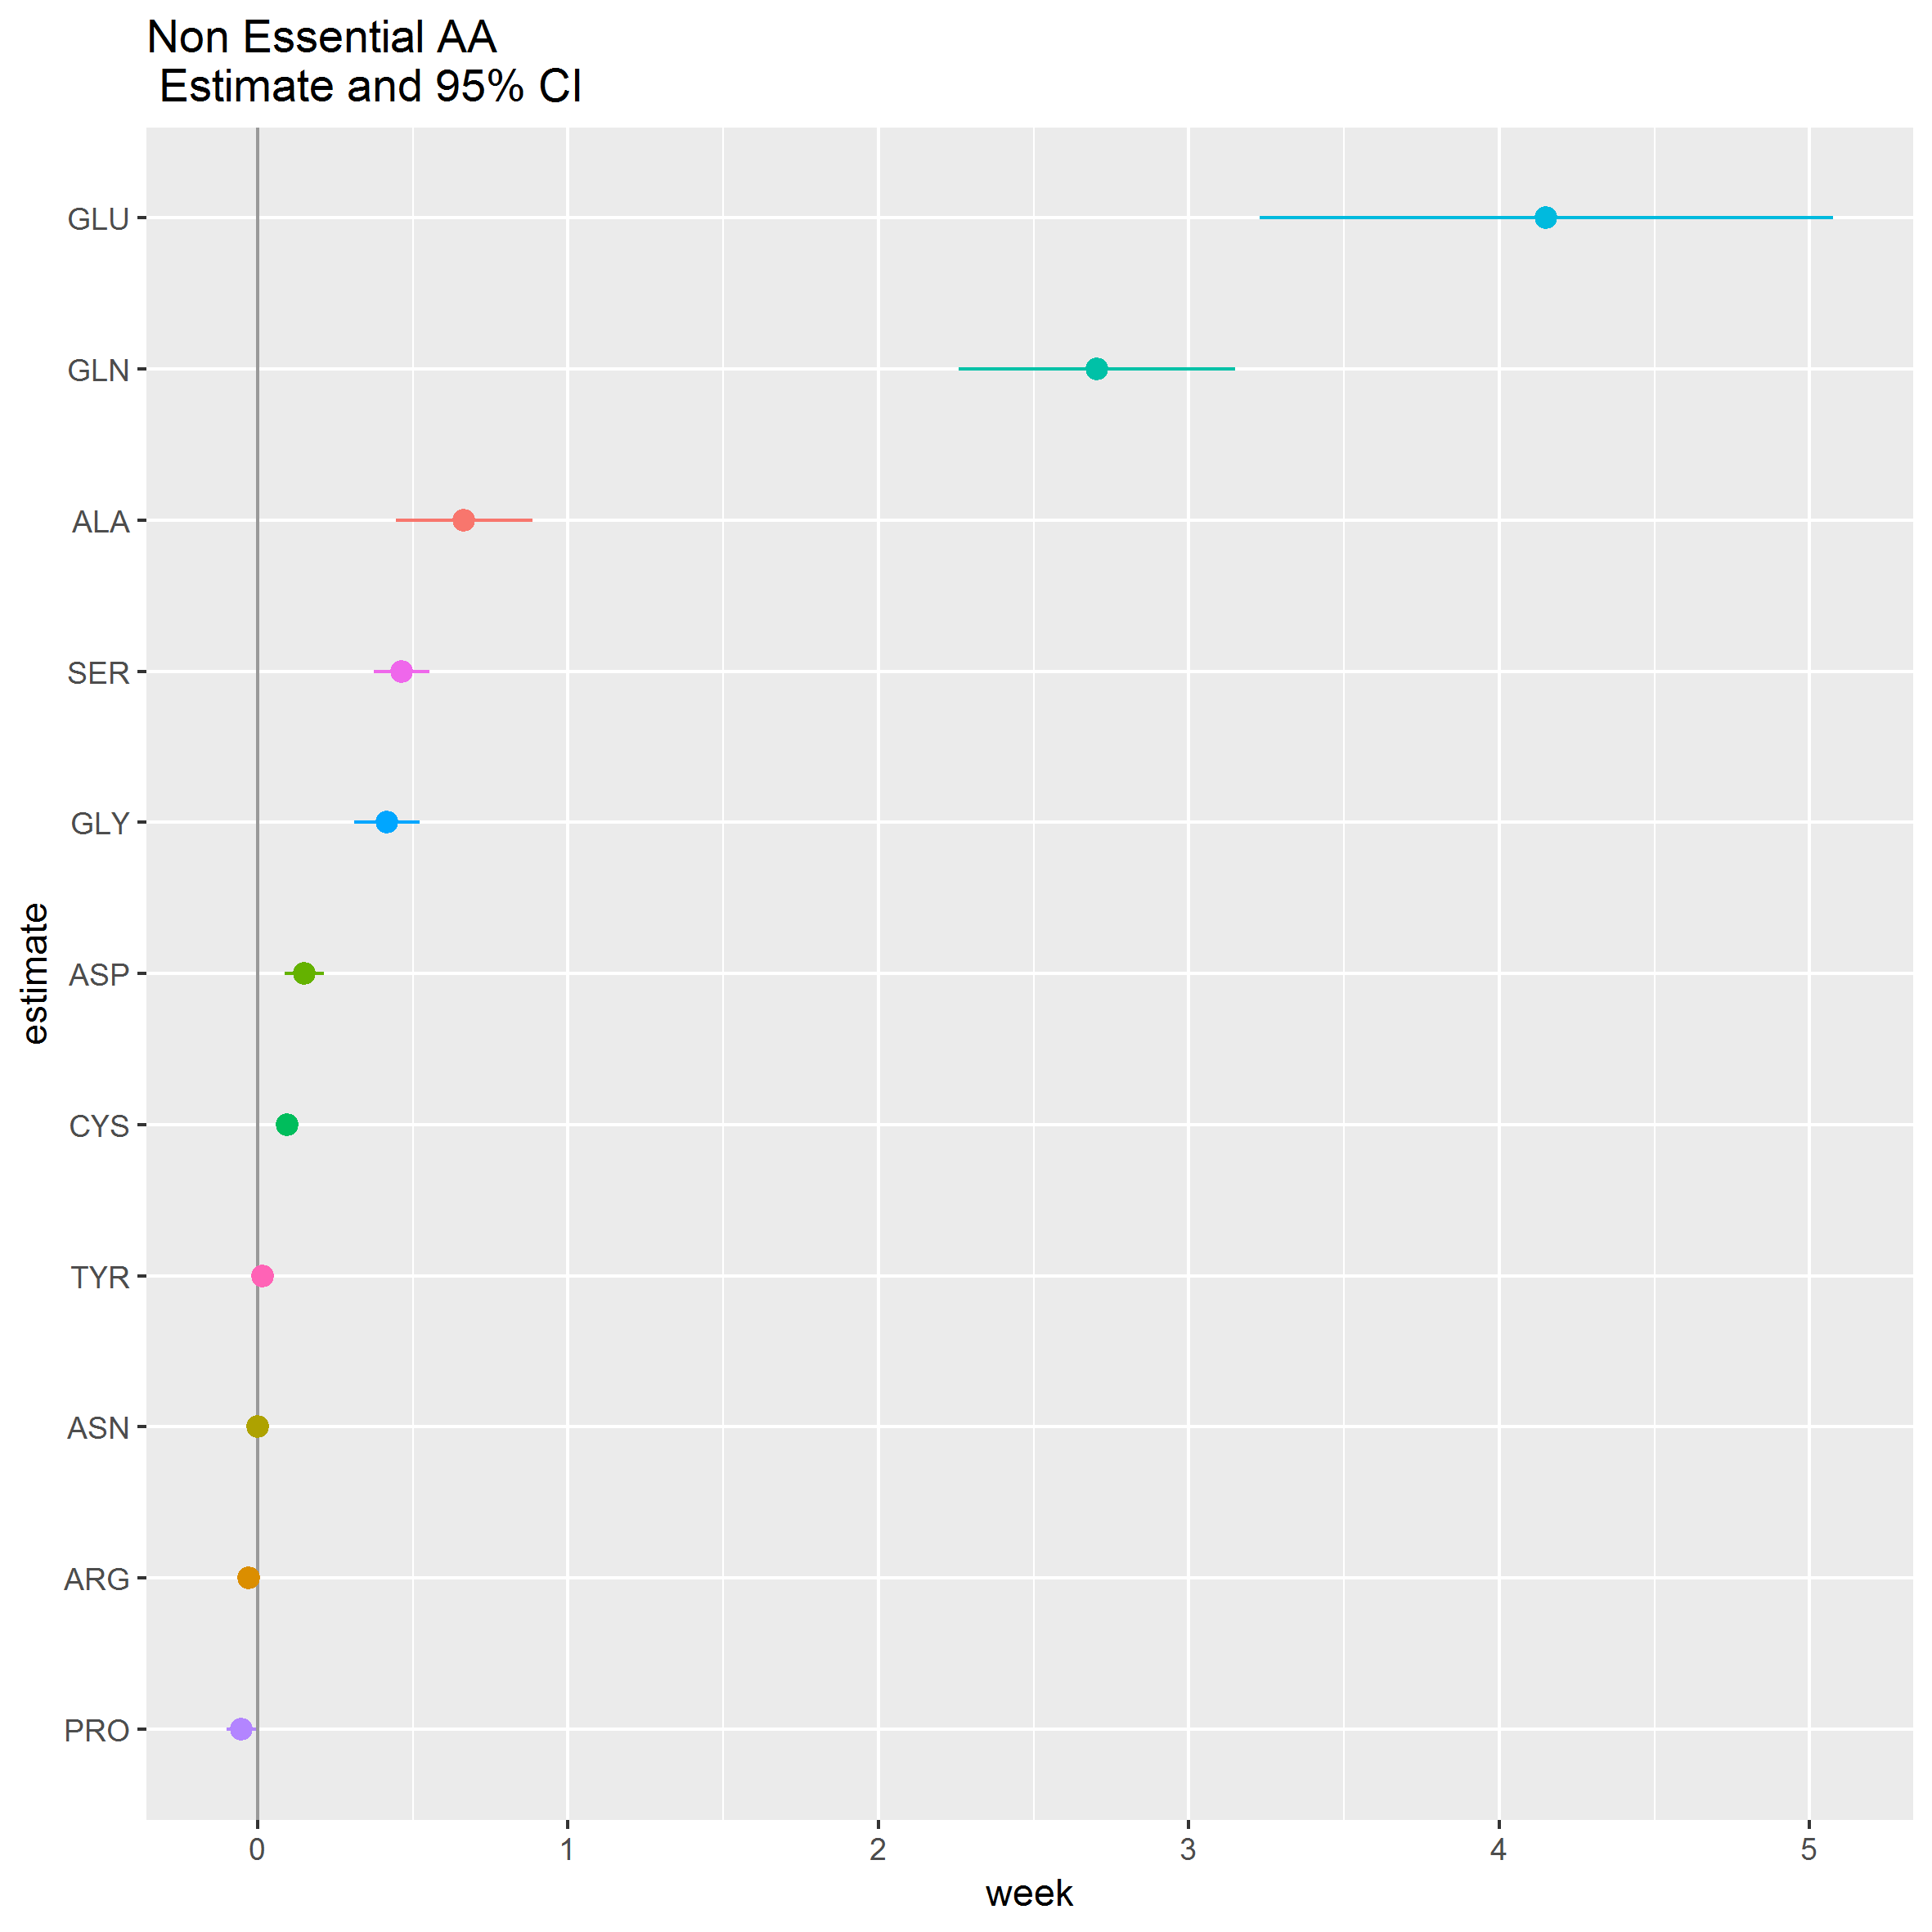
\includegraphics[width= \textwidth]{../week/NEAA_W_coeff.png}
  \caption{}
\end{figure}


\section{}

%\bibliographystyle{plain}
%\bibliography{thebibliography}

%\begin{thebibliography}{1}

%\bibitem{python} Python Software Foundation. Python Language Reference, version 3.6 Available at http://www.python.org.

%\bibitem{COBRApy} COBRApy: COnstraints-Based Reconstruction and Analysis for Python,
%Ali Ebrahim, Joshua A. Lerman, Bernhard O. Palsson, and Daniel R. Hyduke,
%BMC Systems Biology, 2013, 7:74.

%\end{thebibliography}

\end{document}
This is never printed
